\Opensolutionfile{solutions}[ex]
\section*{Exercises}

\begin{enumialphparenastyle}

\begin{ex}  Find the matrix for the linear transformation which
rotates every vector in $\R^{2}$ through an angle of $\pi /3$.
\begin{sol}
$\begin{mymatrix}{cc}
\cos \tup{
\frac{\pi }{3}} & -\sin \tup{\frac{\pi }{3}} \\
\sin \tup{\frac{\pi }{3}} & \cos \tup{\frac{\pi }{3}}%
\end{mymatrix} = \begin{mymatrix}{cc}
\frac{1}{2} & -\frac{1}{2}\sqrt{3} \\
\frac{1}{2}\sqrt{3} & \frac{1}{2}
\end{mymatrix} $
\end{sol}
\end{ex}


\begin{ex} Find the matrix for the linear transformation which rotates every
vector in $\R^{2}$ through an angle of $\pi /4$.
\begin{sol}
$\begin{mymatrix}{cc}
\cos \tup{\frac{\pi }{4}} & -\sin \tup{\frac{\pi }{4}} \\
\sin \tup{\frac{\pi }{4}} & \cos \tup{\frac{\pi }{4}}
\end{mymatrix} = \begin{mymatrix}{cc}
\frac{1}{2}\sqrt{2} & -\frac{1}{2}\sqrt{2} \\
\frac{1}{2}\sqrt{2} & \frac{1}{2}\sqrt{2}
\end{mymatrix} $
\end{sol}
\end{ex}

\begin{ex} Find the matrix for the linear transformation which rotates every
vector in $\R^{2}$ through an angle of $-\pi /3$.
\begin{sol}
$\begin{mymatrix}{cc}
\cos \tup{-\frac{\pi }{3}} & -\sin \tup{-\frac{\pi }{3}} \\
\sin \tup{-\frac{\pi }{3}} & \cos \tup{-\frac{\pi }{3}}
\end{mymatrix} = \begin{mymatrix}{cc}
\frac{1}{2} & \frac{1}{2}\sqrt{3} \\
-\frac{1}{2}\sqrt{3} & \frac{1}{2}
\end{mymatrix} $
\end{sol}
\end{ex}

\begin{ex} Find the matrix for the linear transformation which rotates every
vector in $\R^{2}$ through an angle of $2\pi /3$.
\begin{sol}
$\begin{mymatrix}{cc}
\cos \tup{\frac{2\pi }{3}} & -\sin \tup{\frac{2\pi }{3}} \\
\sin \tup{\frac{2\pi }{3}} & \cos \tup{\frac{2\pi }{3}}
\end{mymatrix} = \begin{mymatrix}{cc}
-\frac{1}{2} & -\frac{1}{2}\sqrt{3} \\
\frac{1}{2}\sqrt{3} & -\frac{1}{2}
\end{mymatrix} $
\end{sol}
\end{ex}

\begin{ex} Find the matrix for the linear transformation which rotates every
vector in $\R^{2}$ through an angle of $\pi /12$. \textbf{Hint:\ }
Note that $\pi /12=\pi /3-\pi /4$.
\begin{sol}
\begin{eqnarray*}
&&\begin{mymatrix}{cc}
\cos \tup{\frac{\pi }{3}}  & -\sin \tup{\frac{\pi }{3}}  \\
\sin \tup{\frac{\pi }{3}}  & \cos \tup{\frac{\pi }{3}}
\end{mymatrix} \begin{mymatrix}{cc}
\cos \tup{-\frac{\pi }{4}}  & -\sin \tup{-\frac{\pi }{4}}
\\
\sin \tup{-\frac{\pi }{4}}  & \cos \tup{-\frac{\pi }{4}}
\end{mymatrix}  \\
&=&\begin{mymatrix}{cc}
\frac{1}{4}\sqrt{2}\sqrt{3}+\frac{1}{4}\sqrt{2} & \frac{1}{4}\sqrt{2}-\frac{1
}{4}\sqrt{2}\sqrt{3} \\
\frac{1}{4}\sqrt{2}\sqrt{3}-\frac{1}{4}\sqrt{2} & \frac{1}{4}\sqrt{2}\sqrt{3}
+\frac{1}{4}\sqrt{2}
\end{mymatrix}
\end{eqnarray*}
\end{sol}
\end{ex}

\begin{ex} Find the matrix for the linear transformation which rotates every
vector in $\R^{2}$ through an angle of $2\pi /3$ and then reflects
across the $x$ axis.
\begin{sol}
\[
\begin{mymatrix}{rr}
1 & 0 \\
0 & -1
\end{mymatrix} \begin{mymatrix}{cc}
\cos \tup{\frac{2\pi }{3}}  & -\sin \tup{\frac{2\pi }{3}}
\\
\sin \tup{\frac{2\pi }{3}}  & \cos \tup{\frac{2\pi }{3}}
\end{mymatrix} = \begin{mymatrix}{cc}
-\frac{1}{2} & -\frac{1}{2}\sqrt{3} \\
-\frac{1}{2}\sqrt{3} & \frac{1}{2}
\end{mymatrix}
\]
\end{sol}
\end{ex}

\begin{ex} Find the matrix for the linear transformation which rotates every
vector in $\R^{2}$ through an angle of $\pi /3$ and then reflects
across the $x$ axis.
\begin{sol}
\[
\begin{mymatrix}{rr}
1 & 0 \\
0 & -1
\end{mymatrix} \begin{mymatrix}{cc}
\cos \tup{\frac{\pi }{3}}  & -\sin \tup{\frac{\pi }{3}}  \\
\sin \tup{\frac{\pi }{3}}  & \cos \tup{\frac{\pi }{3}}
\end{mymatrix} = \begin{mymatrix}{cc}
\frac{1}{2} & -\frac{1}{2}\sqrt{3} \\
-\frac{1}{2}\sqrt{3} & -\frac{1}{2}
\end{mymatrix}
\]
\end{sol}
\end{ex}

\begin{ex} Find the matrix for the linear transformation which rotates every
vector in $\R^{2}$ through an angle of $\pi /4$ and then reflects
across the $x$ axis.
\begin{sol}
\[
\begin{mymatrix}{rr}
1 & 0 \\
0 & -1
\end{mymatrix} \begin{mymatrix}{cc}
\cos \tup{\frac{\pi }{4}}  & -\sin \tup{\frac{\pi }{4}}  \\
\sin \tup{\frac{\pi }{4}}  & \cos \tup{\frac{\pi }{4}}
\end{mymatrix}  =  \begin{mymatrix}{cc}
\frac{1}{2}\sqrt{2} & -\frac{1}{2}\sqrt{2} \\
-\frac{1}{2}\sqrt{2} & -\frac{1}{2}\sqrt{2}
\end{mymatrix}
\]
\end{sol}
\end{ex}

\begin{ex} Find the matrix for the linear transformation which rotates every
vector in $\R^{2}$ through an angle of $\pi /6$ and then reflects
across the $x$ axis followed by a reflection across the $y$ axis.
\begin{sol}
\[
\begin{mymatrix}{rr}
-1 & 0 \\
0 & 1
\end{mymatrix} \begin{mymatrix}{cc}
\cos \tup{\frac{\pi }{6}}  & -\sin \tup{\frac{\pi }{6}}  \\
\sin \tup{\frac{\pi }{6}}  & \cos \tup{\frac{\pi }{6}}
\end{mymatrix} = \begin{mymatrix}{cc}
-\frac{1}{2}\sqrt{3} & \frac{1}{2} \\
\frac{1}{2} & \frac{1}{2}\sqrt{3}
\end{mymatrix}
\]
\end{sol}
\end{ex}

\begin{ex} Find the matrix for the linear transformation which reflects every
vector in $\R^{2}$ across the $x$ axis and then rotates every vector
through an angle of $\pi /4$.
\begin{sol}
\[
\begin{mymatrix}{cc}
\cos \tup{\frac{\pi }{4}}  & -\sin \tup{\frac{\pi }{4}}  \\
\sin \tup{\frac{\pi }{4}}  & \cos \tup{\frac{\pi }{4}}
\end{mymatrix} \begin{mymatrix}{rr}
1 & 0 \\
0 & -1
\end{mymatrix} = \begin{mymatrix}{cc}
\frac{1}{2}\sqrt{2} & \frac{1}{2}\sqrt{2} \\
\frac{1}{2}\sqrt{2} & -\frac{1}{2}\sqrt{2}
\end{mymatrix}
\]
\end{sol}
\end{ex}

\begin{ex} Find the matrix for the linear transformation which reflects every
vector in $\R^{2}$ across the $y$ axis and then rotates every vector
through an angle of $\pi /4$.
\begin{sol}
\[
\begin{mymatrix}{cc}
\cos \tup{\frac{\pi }{4}}  & -\sin \tup{\frac{\pi }{4}}  \\
\sin \tup{\frac{\pi }{4}}  & \cos \tup{\frac{\pi }{4}}
\end{mymatrix} \begin{mymatrix}{rr}
-1 & 0 \\
0 & 1
\end{mymatrix} = \begin{mymatrix}{cc}
-\frac{1}{2}\sqrt{2} & -\frac{1}{2}\sqrt{2} \\
-\frac{1}{2}\sqrt{2} & \frac{1}{2}\sqrt{2}
\end{mymatrix}
\]
\end{sol}
\end{ex}

\begin{ex} Find the matrix for the linear transformation which reflects every
vector in $\R^{2}$ across the $x$ axis and then rotates every vector
through an angle of $\pi /6$.
\begin{sol}
\[
\begin{mymatrix}{cc}
\cos \tup{\frac{\pi }{6}}  & -\sin \tup{\frac{\pi }{6}}  \\
\sin \tup{\frac{\pi }{6}}  & \cos \tup{\frac{\pi }{6}}
\end{mymatrix} \begin{mymatrix}{rr}
1 & 0 \\
0 & -1
\end{mymatrix} =  \begin{mymatrix}{cc}
\frac{1}{2}\sqrt{3} & \frac{1}{2} \\
\frac{1}{2} & -\frac{1}{2}\sqrt{3}
\end{mymatrix}
\]
\end{sol}
\end{ex}

\begin{ex} Find the matrix for the linear transformation which reflects every
vector in $\R^{2}$ across the $y$ axis and then rotates every vector
through an angle of $\pi /6$.
\begin{sol}
\[
\begin{mymatrix}{cc}
\cos \tup{\frac{\pi }{6}}  & -\sin \tup{\frac{\pi }{6}}  \\
\sin \tup{\frac{\pi }{6}}  & \cos \tup{\frac{\pi }{6}}
\end{mymatrix} \begin{mymatrix}{rr}
-1 & 0 \\
0 & 1
\end{mymatrix} = \begin{mymatrix}{cc}
-\frac{1}{2}\sqrt{3} & -\frac{1}{2} \\
-\frac{1}{2} & \frac{1}{2}\sqrt{3}
\end{mymatrix}
\]
\end{sol}
\end{ex}

\begin{ex} Find the matrix for the linear transformation which rotates every
vector in $\R^{2}$ through an angle of $5\pi /12$. \textbf{Hint:\ }
Note that $5\pi /12=2\pi /3-\pi /4$.
\begin{sol}
\[
\begin{mymatrix}{cc}
\cos \tup{\frac{2\pi }{3}} & -\sin \tup{\frac{2\pi }{3}} \\
\sin \tup{\frac{2\pi }{3}} & \cos \tup{\frac{2\pi }{3}}
\end{mymatrix} \begin{mymatrix}{cc}
\cos \tup{-\frac{\pi }{4}} & -\sin \tup{-\frac{\pi }{4}} \\
\sin \tup{-\frac{\pi }{4}} & \cos \tup{-\frac{\pi }{4}}
\end{mymatrix} = 
\]
\[
\begin{mymatrix}{cc}
\frac{1}{4}\sqrt{2}\sqrt{3}-\frac{1}{4}\sqrt{2} & -\frac{1}{4}\sqrt{2}\sqrt{3
}-\frac{1}{4}\sqrt{2} \\
\frac{1}{4}\sqrt{2}\sqrt{3}+\frac{1}{4}\sqrt{2} & \frac{1}{4}\sqrt{2}\sqrt{3}
-\frac{1}{4}\sqrt{2}
\end{mymatrix}
\]
Note that it doesn't matter about the order in this case.
\end{sol}
\end{ex}

\begin{ex} Find the matrix of the linear transformation which rotates every
vector in $\R^{3}$ counter clockwise about the $z$ axis when viewed
from the positive $z$ axis through an angle of 30$^{\circ }$ and then
reflects through the $xy$ plane.
\begin{sol}
\[
\begin{mymatrix}{rrr}
1 & 0 & 0 \\
0 & 1 & 0 \\
0 & 0 & -1
\end{mymatrix} \begin{mymatrix}{ccc}
\cos \tup{\frac{\pi }{6}}  & -\sin \tup{\frac{\pi }{6}}  & 0
\\
\sin \tup{\frac{\pi }{6}}  & \cos \tup{\frac{\pi }{6}}  & 0
\\
0 & 0 & 1
\end{mymatrix} = \begin{mymatrix}{ccc}
\frac{1}{2}\sqrt{3} & -\frac{1}{2} & 0 \\
\frac{1}{2} & \frac{1}{2}\sqrt{3} & 0 \\
0 & 0 & -1
\end{mymatrix}
\]
\end{sol}
\end{ex}
 
\begin{ex} Let $\vect{u}=\begin{mymatrix}{r}
a \\
b
\end{mymatrix} $ be a unit vector in $\R^{2}$. Find the matrix
\index{reflection!across a given vector} which reflects all vectors across
this vector, as shown in the following picture. 

\begin{center}
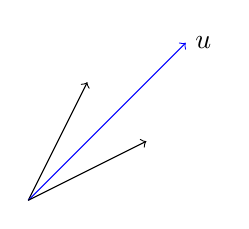
\begin{tikzpicture}
\draw[->](0,0)--(0.75,1.5);
\draw[blue, ->](0,0)--(2,2);
\draw[->](0,0)--(1.5,0.75);
\node[right] at (2,2){$\vect{u}$};
\end{tikzpicture}
\end{center}


\textbf{Hint:\ }Notice that $\begin{mymatrix}{r}
a \\
b
\end{mymatrix} =\begin{mymatrix}{c}
\cos \theta  \\
\sin \theta 
\end{mymatrix} $ for some $\theta$. First rotate through $-\theta$. Next reflect through the $x$ axis. Finally rotate
through $\theta$. 
\begin{sol}
\begin{eqnarray*}
&&\begin{mymatrix}{cc}
\cos \tup{\theta } & -\sin \tup{\theta } \\
\sin \tup{\theta } & \cos \tup{\theta }
\end{mymatrix} \begin{mymatrix}{rr}
1 & 0 \\
0 & -1
\end{mymatrix} \begin{mymatrix}{cc}
\cos \tup{-\theta } & -\sin \tup{-\theta } \\
\sin \tup{-\theta } & \cos \tup{-\theta }
\end{mymatrix} \\
&=& \begin{mymatrix}{cc}
\cos ^{2}\theta -\sin ^{2}\theta & 2\cos \theta \sin \theta \\
2\cos \theta \sin \theta & \sin ^{2}\theta -\cos ^{2}\theta%
\end{mymatrix}
\end{eqnarray*}
Now to write in terms of $\tup{a,b}$, note that $a/\sqrt{a^{2}+b^{2}
}=\cos \theta ,b/\sqrt{a^{2}+b^{2}}=\sin \theta$. Now plug this in to the
above. The result is
\[
\begin{mymatrix}{cc}
\frac{a^{2}-b^{2}}{a^{2}+b^{2}} & 2\frac{ab}{a^{2}+b^{2}} \\
2\frac{ab}{a^{2}+b^{2}} & \frac{b^{2}-a^{2}}{a^{2}+b^{2}}
\end{mymatrix} =\frac{1}{a^{2}+b^{2}}\begin{mymatrix}{cc}
a^{2}-b^{2} & 2ab \\
2ab & b^{2}-a^{2}
\end{mymatrix}
\]
Since this is a unit vector, $a^{2}+b^{2}=1$ and so you get
\[
\begin{mymatrix}{cc}
a^{2}-b^{2} & 2ab \\
2ab & b^{2}-a^{2}
\end{mymatrix}
\]
\end{sol}
\end{ex}

\end{enumialphparenastyle}